\section{Własności wykorzystywanych materiałów}
\label{subart:thzmat}
Kluczowymi procesami odpowiedzialnymi za wartość przenikalności elektrycznej ciał stałych dla niskich częstotliwości terahercowych, określanych niekiedy jako subterahercowe, są model elektronów swobodnych Drudego (patrz sekcja \ref{subart:lorenz-drude}) i~relaksacja Debye'a. Dla częstotliwości bliższych dalekiej podczerwieni podstawowe znaczenie mają optyczne fonony - skwantowane mody drgań sieci krystalicznej. Typowe wartości współczynnika załamania polimerów mieszczą się w~przedziale $n \in (1.4;1.5)$, a~dla półprzewodników $n\in (3.1;3.5)$. W~obu wypadkach charakteryzują się niewielką dyspersją. Wypolerowane powierzchnie metalowe są wykorzystywane jako zwierciadła o~współczynniku odbicia $R\approx 0.99$ \cite{lee2009principles}.

W układach omawianych w~poniższym rozdziale wykorzystywane są złoto i~arsenek galu, dlatego ich własności omówione zostaną bardziej szczegółowo. Wszystkie przewodniki, w~tym złoto, ze względu na czasy relaksacji rzędu $10^{-14}$s charakteryzują się niemal bezdyspersyjną przewodnością. W związku z~tym, równanie (\ref{eq:lorenz-drude}) możemy zapisać w~prostszej postaci
\begin{equation}
	\varepsilon(\omega)=\varepsilon_{\infty}+i \frac{\sigma_0}{\varepsilon_0 \omega},
	\label{eq:eps-met-thz}
\end{equation}
gdzie przez $\sigma_0$ oznaczona została przewodność. Dla złota w~warunkach normalnych $\sigma_0=45.2 \frac{S}{\mu m}$.   Ze względu na znacznie większą wartość bezwzględną części urojonej przenikalności elektrycznej od rzeczywistej, dla zakresu subterahercowego powyższe równanie (\ref{eq:eps-met-thz}) możemy dalej uprościć do postaci
\begin{equation}
	\varepsilon(\omega) \approx i~\frac{\sigma_0}{\varepsilon_0 \omega}.
	\label{eq:eps-met-thz-app}
\end{equation}

\begin{figure}[tb]
	\begin{subfigure}{.45\textwidth}
		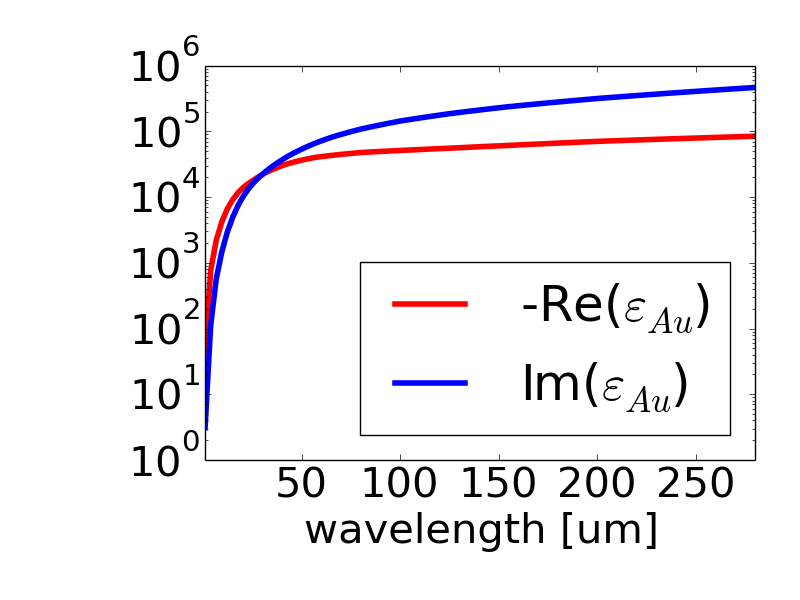
\includegraphics[width=\textwidth]{images/aueps.png}
		\caption{}
		\label{fig:aueps}
	\end{subfigure}
	\begin{subfigure}{.45\textwidth}
		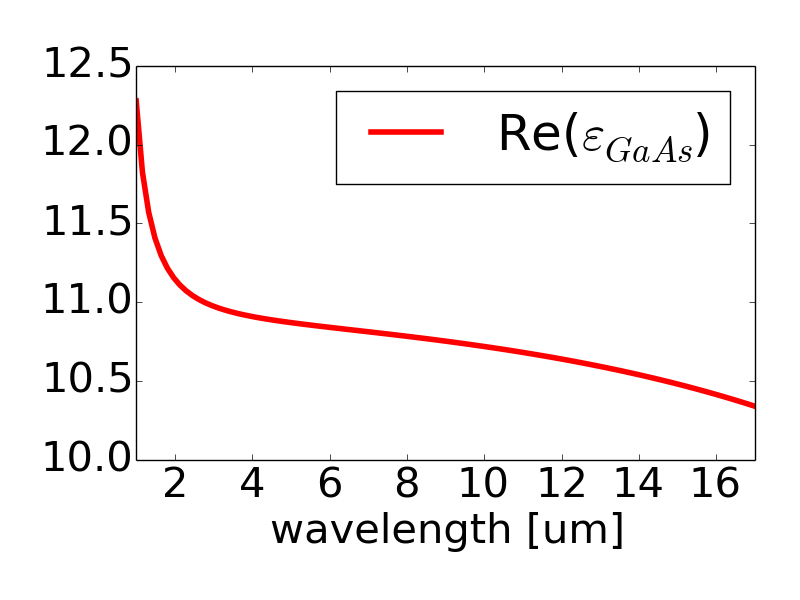
\includegraphics[width=\textwidth]{images/gaaseps.png}
		\caption{}
		\label{fig:gaaseps}
	\end{subfigure}
	\caption{Zależność przenikalności elektrycznej od długości fali dla (a)~$Au$~\cite{Hagemann:75}, (b)~$GaAs$~\cite{skauli2003improved}}
\end{figure}

Różnica wartości bezwzględnej części rzeczywistej i~urojonej przenikalności elektrycznej złota zmniejsza się wraz ze wzrostem częstotliwości. Dla $f=2$~THz moduł części rzeczywistej jest ok. 5 razy mniejszy od modułu części urojonej. Część rzeczywista przenikalności elektrycznej dla fal optycznych i dłuższych jest ujemna, a jej moduł zmienia się od kilkudziesięciu do ponad $10^4$ w zakresie od podczerwieni do obszaru terahercowego. Ze względu na dominujący charakter części urojonej związanej z~przewodnictwem, eksperymentalne wyznaczenie przenikalności elektrycznej jest bardzo trudne. Eksperymentalne wyznaczenie części rzeczywistej $\varepsilon_{\textrm{Au}}$ prowadzone jest jedynie dla częstotliwości powyżej $1$~THz~(długości fali poniżej ok. $300$~$\mu$m)~\cite{ordal1983optical}\footnote{Powyższa analiza prawdziwa jest dla eksperymentów prowadzonych w~temperaturze pokojowej. Obniżenie temperatury do~$T=$80K powoduje wzrost przewodności złota do $\sigma_0=208\frac{S}{\mu m}$. W temperaturach kriogenicznych w~cienkich warstwach złota dominujący wpływ na przewodność może mieć rozpraszanie elektronów na defektach struktury~\cite{lide2009crc}}. Zależność $\varepsilon$ od długości fali została przedstawiona na wykresie \ref{fig:aueps}. 

Symulacje opisywane w~poniższym rozdziale prowadzone są z~maksymalną rozdzielczością $0.5$~$\mu$m na punkt obliczeniowy, natomiast głębokość naskórkowa dla $1$~THz, $\delta=74.9$~nm~\cite{lee2009principles}. Mała głębokość naskórkowa w~porównaniu do długości fali oraz rozmiaru siatki przyjętej w~obliczeniach uprawnia do przybliżenia złota przez doskonały przewodnik. 

W przeciwieństwie do złota, warstwy $GaAs$ w~zakresie THz mogą być traktowane jako bezstratne. Charakteryzują się one również słabą dyspersją, a w~przypadku obliczeń prowadzonych dla wąskiego zakresu długości fali, wartość przenikalności elektrycznej może być traktowana jako stała. Warto jednak zwrócić uwagę na to, że warstwy $GaAs$ uzyskiwane w~wyniku epitaksji z~wiązki molekularnej poddawane są zazwyczaj procesowi wygrzewania w~celu ich wygładzenia lub eliminacji zanieczyszczeń. Proces ten może mieć jednak znaczący wpływ na koncentrację elektronów w~paśmie przewodnictwa, co może istotnie zmienić właściwości elektromagnetyczne tego materiału~\cite{zhang2009annealing}. Zależność przenikalności elektrycznej od długości fali dla $GaAs$ przedstawia wykres na rysunku \ref{fig:gaaseps}.
